\textbf{Model uczony na stałej krzywiźnie wierzechołków}

\begin{figure}[ht]
	\centering
	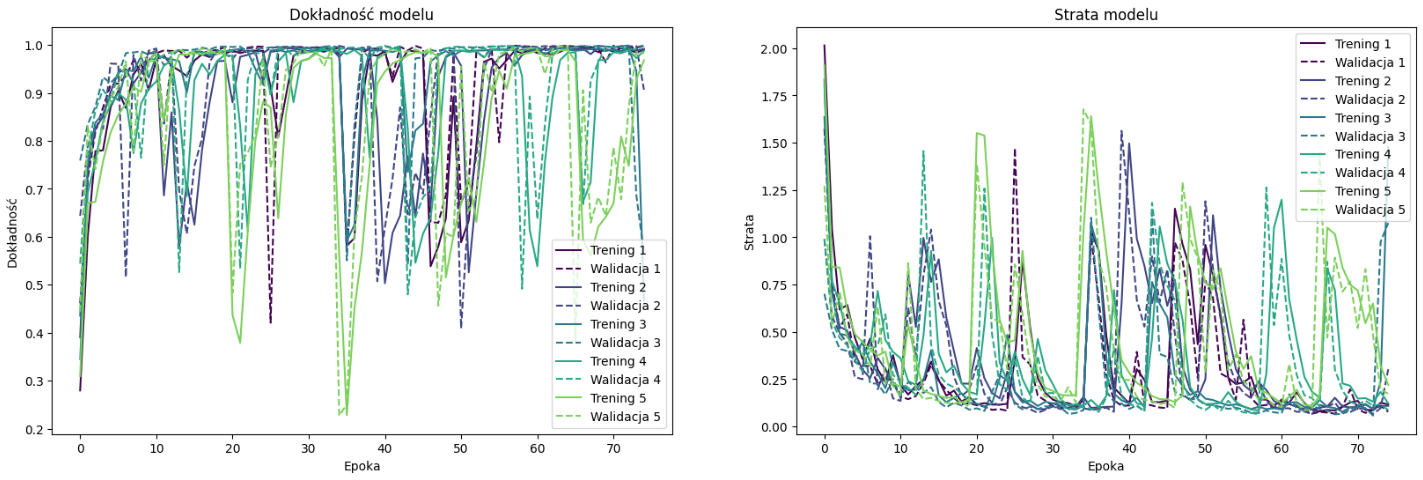
\includegraphics[height=5.5cm]{resources/tests/images/v2/crossvalid_img.png}
	\caption{Wyniki testów dla modelu z walidacją krzyżową i stałą krzywizną wierzechołków}
	\label{Fig:tests-cv-1}
\end{figure}
\FloatBarrier

\begin{figure}[ht]
	\centering
	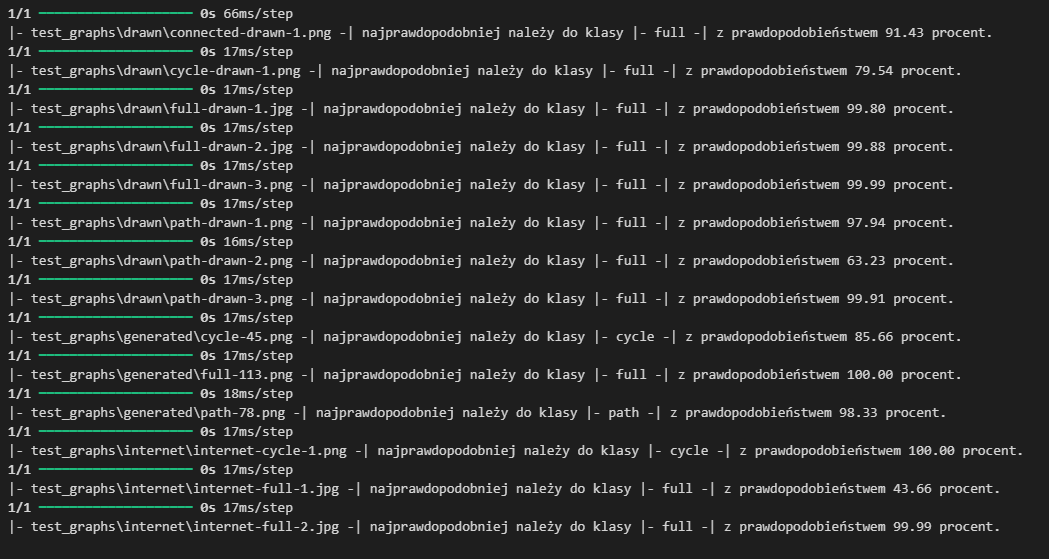
\includegraphics[height=7cm]{resources/tests/images/v2/crossvalid_txt.png}
	\caption{Klasyfikacja obrazów zewnętrznych dla modelu z walidacją krzyżową i stałą krzywizną wierzechołków}
	\label{Fig:tests-cv-2}
\end{figure}
\FloatBarrier

\textbf{Model uczony na losowej krzywiźnie wierzechołków}

W przypadku modelu z walidacją krzyżową, uczonego na grafach z 4 wierzchołkami,
dokładność wzrasta gwałtownie na początku treningu,
osiągając wartości powyżej 0.8 już po około 10 epokach.
Dokładność stabiliziuje się w okolicach 90\%, ale mimo to widać pewne fluktuacje, zwłaszacza na danych walidacyjnych.
Możliwe do zaobserowania są regularne spadki dokładności w niektórych epokach,
co może wynikać z niestabilnego treningu lub problemów modelu w generalizacji dla niektórych danych walidacyjncyh.

Dla straty modelu można zaobserować spadek w pierwszych 10 epokach, co mogłoby wskazywać na szybkie uczenie się modelu.
Zaraz po nim, następuje stabilizacja na niskim poziomie, z pojedynczymi skokami, głównie na zbiorze walidacyjnym.
Nieregularne wzrosty straty, podobnie jak w przypadku dokładności, mogą wskazywać na problemy z przeuczeniem.

\begin{figure}[ht]
	\centering
	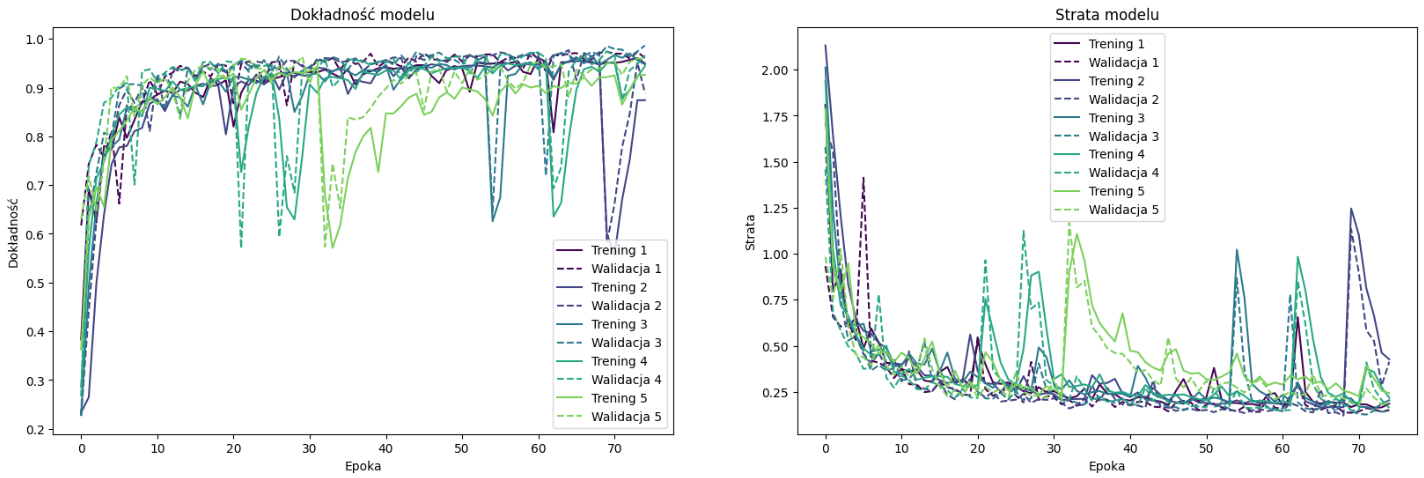
\includegraphics[height=5.5cm]{resources/tests/images/v3/crossvalid_img.png}
	\caption{Wyniki testów dla modelu z walidacją krzyżową i losową krzywizną wierzchołków}
	\label{Fig:tests-cv-1}
\end{figure}
\FloatBarrier

Podsumowując, ten wariant modelu generalnie uczy się poprawnie, dzięki czemu osiąga wysoką dokładność i niską stratę.
Fluktuacje jakie występują w wynikach, szczególnie na danych walidacyjnych,
sugerują jednak potencjalne problemy z generalizacją, co może być wynikiem niestabilności modelu,
przeuczenia modelu, lub trudności w rozpoznawaniu bardziej złożonych przykładów w danych walidacyjnych.

W przypadku tego modelu, zwiększenie liczby epok, nie przyniosłoby zamierzonych skutków.
Model zbyt szybko się przeucza, a więc większa liczba iteracji nie wpłynęłaby w żaden znaczący sposób na wynik.

% Została podjęta próba ograniczenia przeuczenia poprzez zwiększenie zbioru danych, zmiany liczby epok w modelu
% oraz manipulacji współczynnikami dropout i regularyzacji.
% W każdym przypadku model zwracał niezadowalające wyniki wynoszące 100\% po jednej z początkowych iteracji.

\begin{figure}[ht]
	\centering
	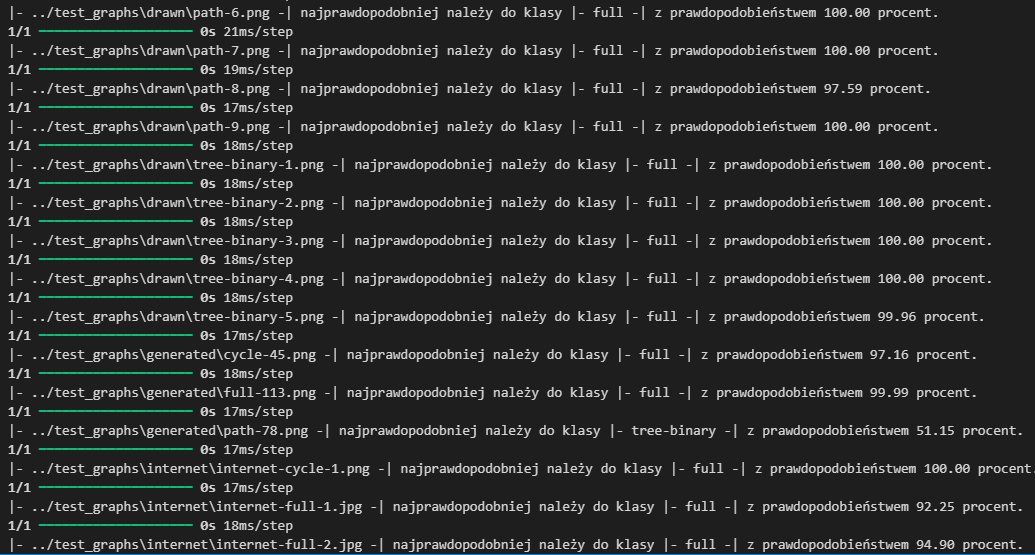
\includegraphics[height=7cm]{resources/tests/images/v3/crossvalid_txt.png}
	\caption{Klasyfikacja obrazów zewnętrznych dla modelu z walidacją krzyżową i losową krzywizną wierzchołków}
	\label{Fig:tests-cv-2}
\end{figure}
\FloatBarrier

Z powodu przeuczenia model nie radził sobie z zewnętrznymi obrazkami testowymi.
Większość grafów określił jako grafy pełne, a jedną ze scieżek jako drzewo binarne,
co nie jest zgodne ze stanem rzeczywistym.